%%%%%%%%%%%%%%%%%%%%%%%%%%%%%%%%%%%%%%%%%%%%%%%%%%%%%%%%%%%%%%%%%%
%%%%%%%% ICML 2015 EXAMPLE LATEX SUBMISSION FILE %%%%%%%%%%%%%%%%%
%%%%%%%%%%%%%%%%%%%%%%%%%%%%%%%%%%%%%%%%%%%%%%%%%%%%%%%%%%%%%%%%%%

% Use the following line _only_ if you're still using LaTeX 2.09.
%\documentstyle[icml2015,epsf,natbib]{article}
% If you rely on Latex2e packages, like most moden people use this:
\documentclass{article}

% use Times
\usepackage{times}
% For figures
\usepackage{graphicx} % more modern
%\usepackage{epsfig} % less modern
\usepackage{subfigure} 

% For citations
\usepackage{natbib}

% For algorithms
\usepackage{algorithm}
\usepackage{algorithmic}
\usepackage{algorithm2e}
\usepackage{multirow}

% As of 2011, we use the hyperref package to produce hyperlinks in the
% resulting PDF.  If this breaks your system, please commend out the
% following usepackage line and replace \usepackage{icml2015} with
% \usepackage[nohyperref]{icml2015} above.
\usepackage{hyperref}

% Packages hyperref and algorithmic misbehave sometimes.  We can fix
% this with the following command.
\newcommand{\theHalgorithm}{\arabic{algorithm}}

% Employ the following version of the ``usepackage'' statement for
% submitting the draft version of the paper for review.  This will set
% the note in the first column to ``Under review.  Do not distribute.''
\usepackage{icml2015} 

% Employ this version of the ``usepackage'' statement after the paper has
% been accepted, when creating the final version.  This will set the
% note in the first column to ``Proceedings of the...''
%\usepackage[accepted]{icml2015}


% The \icmltitle you define below is probably too long as a header.
% Therefore, a short form for the running title is supplied here:
\icmltitlerunning{Submission and Formatting Instructions for ICML 2015}

\begin{document} 

\twocolumn[
\icmltitle{Measuring the effect of immigration on mood expressed on 
Twitter}

% It is OKAY to include author information, even for blind
% submissions: the style file will automatically remove it for you
% unless you've provided the [accepted] option to the icml2015
% package.
\icmlauthor{Rojin Babayan}{rbabayan@hawk.iit.edu}
\icmladdress{Illinois Institute of Technology, 
            3300 South Federal Street
            Chicago, IL 60616-3793}
\icmlauthor{Your CoAuthor's Name}{email@coauthordomain.edu}
\icmladdress{Their Fantastic Institute,
            27182 Exp St., Toronto, ON M6H 2T1 CANADA}

% You may provide any keywords that you 
% find helpful for describing your paper; these are used to populate 
% the "keywords" metadata in the PDF but will not be shown in the document
\icmlkeywords{boring formatting information, machine learning, ICML}

\vskip 0.3in
]

\begin{abstract} 
Traditional studies in Social Science and Psychology indicated a higher risk of depression and mood change in immigrants after their immigration. This project studies the impact of immigration on people based on their mood expressed in their tweets on Twitter. The project has two major parts; 1) identifying the immigrants on Twitter and 2) analyze the sentiment of their tweets to study their mood. For the first part we relied on Twitter geo-location meta-data to see if a user has moved from a country to another. And for the second part we built a Logistic Regression classifier that could assign a probability value to each tweet for three trained class labels; anxiety, dejection, and hostility. The results indicate that all class labels generally increase after immigration in our set of identified immigrants. 
\end{abstract} 

\section{Introduction}
\label{Introduction}

Studies in Social Science indicate a higher risk of psychological distress for immigrants. This is illustrated by measuring different features such as suicide rate, self reported psychiatric illness, intake of psychotropic drugs, and desire to leave the new country. With increased popularity of online social networks, a new data source is available for researchers to study psychological and behavioral features of the users. In this project we focus on Twitter and the tweets made by immigrants to analyze how their psychological features represented in their tweets have changed before and after their immigration. The psychological features investigated in this study are dejection, anxiety, and hostility. Twitter is selected as the base of the study primarily because this micro-blogging service provides publicly available and highly frequent large message volume. 

\subsection{Problem Statement}

The primary research question in this project can be phrased as: \textit{How does immigration impact mental state of the immigrants shown in their tweets?} We break down this question into two sub-problems: 
\begin{enumerate}
    \item How can we identify immigrants on Twitter?
    \item How can we analyze the sentiment of the tweets to extract psychological features?
\end{enumerate}
For the first part we relied on geo-locations of the tweets to detect the location of the users and see if they have changed their location for a long time. And for the second part we used a set of manually labeled training data and a Logistic Regression model to analyze the sentiment of the tweets.   

\subsection{Report Structure}
Section 2 focuses on the related work done in this area. This section first illustrates the traditional approaches done in Social Science and Psychology that studied behavioral and mental features of immigrants. Then it lists the efforts in sentiment analysis of the tweets related to other applications. 

Section 3 describes our data collection method and how we identified immigrants on Twitter. Section 4 then explains the Sentiment Analysis part of the project where we look for the moods expressed on tweets made by the identified immigrants. Section 5 then details our 'Difference in Differences' method and how we evaluated the achieved results. Section 6 then lists the concluding remarks as well as potential future directions for this project. 

\section{Related Work}

Researches and studies related to this project can be categorized into three groups; 
\begin{enumerate}
    \item Traditional approaches in Social Science and Psychology that study the impact of immigration on people's mood
    \item Researches done in geo-locating twitter users using the texts of the tweets and tweets' meta-data
    \item Methods to analyze the sentiment of tweets by their contents
\end{enumerate}

\subsection{Traditional Approaches}

An study by World Health Organization (WHO) \cite{who} indicates that the rate of suicide increases between immigrants in the United States. They compared the rate of suicide between people who have immigrated to USA and the people of the native country who have not made the immigration. Figure \ref{suicide-rate} visualizes the results for each studied country. This gives the initial idea that immigration potentially impacts people in term of their psychological features. A similar study \cite{ref3} has been done for immigrants to Canada and argues that the suicide rate in immigrants to Canada have generally increased compared with the suicide rate in their home country. The result suggests that the immigration is likely to cause depression, and anxiety.

\begin{figure}[ht]
\vskip 0.2in
\begin{center}
\centerline{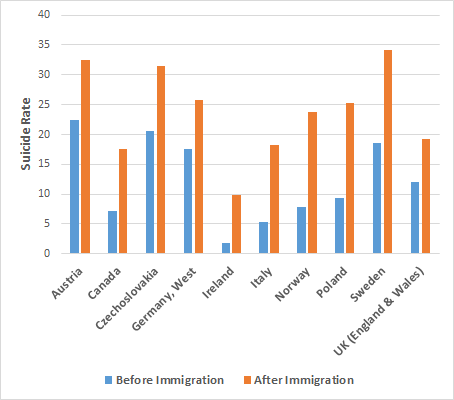
\includegraphics[width=\columnwidth]{Figures/suicide_rate.PNG}}
\caption{Suicide rate per 100,000 people per year between immigrants to the United States compared with their source country}
\label{suicide-rate}
\end{center}
\vskip -0.2in
\end{figure} 

\cite{ref2} studied immigrants in the state of California between 1998 to 2001 and by comparing the suicide rate between immigrants and native people, showed that immigration increased suicide risk. It is argued that the depression is significantly more in divorced and single immigrants than regular immigrants. Moreover, their results indicate that the suicide risk is more for people who have immigrated recently and have a shorter duration of stay. 

In another comprehensive but more recent study \cite{ref4}, the rate of suicide and other parameters impacted by immigration are investigated. Globalization, acculturation and acculturation stress, genetic and environmental factors, urbanization and ethnic density, first or second generation of immigrants, being in adolescents, and being a refugee and asylum seeker, are among the primary parameters discussed in this research that might be the cause of increased suicide and depression rate between immigrants.

Westman et al. \cite{ref5}, categorized the suicides attempts in Sweden based on the place of birth and gender of the person who attempted the suicide. The paper divided the number of attempted suicides to the total population of immigrants for each home country in Sweden, to calculate the rate of suicides for in immigrants based on their home country. The result illustrated that the suicide rate for immigrants from almost every country is more than the native Swedish people. For example the suicide rate of Iranian immigrants in Sweden is twice more than the rate of native people of Sweden, in spite of the fact that the suicide rate of native Iranians living in Iran is half the suicide rate of people from Sweden.

Potochnick et al. \cite{ref6} in yet another study, actively monitored the psychological features of more than 500 Mexican immigrants in the United States and concluded that “After arrival in the United States, migrants had a significantly higher risk for first onset of any depressive or anxiety disorder than did non-immigrant family members of migrants in Mexico.”

Leersnydera et al. \cite{ref16} in a psychological research done manually and based on direct interaction with people and might not be very closely related to our project. Nevertheless, the research revolves around a similar research question as what we are targeting, which is the impact of immigration on one’s psychological feature. The research studied Korean immigrants in the US, and Turkish immigrants in Belgium, with this research assumption that the emotional experiences of people who live together become similar. The result show that an emotional acculturation exist in immigrants.

In conclusion, our literature review in the field of Social Science and Psychology illustrate that immigrants have a higher risk of dejection, depression, and ultimately suicide rate. 

\subsection{Geo-locating Twitter Users}

As part of the project, we need to identify immigrants on Twitter. Therefore, we look into geo-locate tweets and Twitter accounts to see if a user has immigrated or not. This section surveys related work in regard to geo-locating twitter accounts using either the tweets contents or meta-data. 

Cheng et al. \cite{ref7} built a model that successfully estimated the location of 51\% of their testing twitter accounts with the precision of up to 100 miles only based on the textual contents of the tweets. Their approach focuses on the keywords used in tweets that might be associated with a certain location, such as a particular expression, a name of a place, or a name of a local event.

Backstorm et al. \cite{ref8} assumed that the likelihood of friendship with a person decreases with distance, therefore people tend to be located close to their friends. The idea is used in this research to build an algorithm that can anticipate the location of a social network's users based on the location of their friends. It is illustrated that the proposed algorithm outperforms IP-based geolocation.

Amitay et al. \cite{ref9} in their research made this goal to geotag web-pages based on their contents. The approach is to identify keywords in the web-pages that might be associated with different places. However, the challenge targeted in this paper is to resolve ambiguities such as those keywords that might represent different locations, and those that represent both location and non-location meanings. In order to do so, the whole contents of the page is involved in their proposed algorithm to give a score to each potential location for the web-page.

Another research \cite{ref10} on geo-locating web contents on Social Networks studies users’ activities on Foursquare social network where users are able to check in their locations. The study attempts to identify a correlation between the location of the users and their activities to build a framework for a potential recommendation system. Geo-locating the users are solely based on the coordination of the users that they set manually by checking in on the app. This is similar to Twitter’s tweets location. However, Twitter users tend to turn off their location more than Foursquare users.

Foursquare social network has been the subject of another research \cite{ref11} to study the locations of social network users with a goal of building a human mobility pattern. This study also considers the manually set check-ins from the users in social networks for to identify the location of the users. This is how their approach is different from content-based geo-location systems. In another research \cite{ref12} in shaping human mobility based on their locations on social networks, the locations are based on what the users manually set by checking in on social networks such as Foursquare and Facebook. The result of the paper is a proposed model for human mobility patterns in urban metropolitan cities.

A more recent study \cite{ref13} is closely related to our project in term of identifying cross-border mobility of social network users. The research monitors the location of users on location based social networks to capture cross border movements. This interests us as we identify such mobilities with some additional constraints as immigration, and the user would be important for us as an immigrant. Moreover, the research also analyzes twitter accounts and the location of the tweets as well. 

\subsection{Sentiment Analysis on Twitter}

As discussed in Section 1.1, the second sub-problem in this project is to find a methodology to anticipate psychological features of a twitter user, in particular depression by analyzing the sentiment of their tweets. While the goal is for twitter accounts, other proposed approaches that analyzes the sentiment and behaviour of a user based on their web contents might be interested for us as well. Researches done in the fields of Sociology and Psychology are also considered for this purpose.

In a research \cite{ref14} done by Carr et al. the goal is to determine if online tweets represent the idea and opinions of the person who submitted them on twitter. For instance in this research they considered the issue of immigration and concluded that by analyzing the tweets one sent, we are able to determine if they are in favor or opposed to the issue. The analysis and categorizing the tweets however, were done mostly manually to determine if a tweet is positive or negative about the issue.

Kouloumpis et al. \cite{ref17} investigated the application of Sentiment Analysis and Natural Language Processing in Twitter. It is argued that previous researches in this regard explored the use of Part-of-Speech features and were not significantly successful due to the incredible breadth of topic that tweets of a user cover. Therefore, they focused on hashtags used in tweets to mine the sentiment of the tweets, besides lexicon, n-gram, and Part-of-Speech features. The combination of all features resulted in the best performance in term of accuracy based on a training data.

Agarwal et al. \cite{ref15} have done a study in sentiment analysis of tweets. The proposed methodology has three major phases; preprocessing, scoring, and design of a Tree Kernel. The preprocessing is done to organize emoticons, URLs, user mentions, and acronyms such as LOL and gr8. The second phase is to score each word based on being positive or negative using a dictionary of 8000 words that are already scored and WordNet. Finally, they build a tree of each tweet and score a tweet based on a large list of proposed features.

Bollen et al. \cite{ref18} in their research to find the mood of tweets, used profile of Mood States psychometric instrument which measures six individual dimensions of mood (Tension, Depression, Anger, Vigour, Fatigue, Confusion). After data preparation and normalizing tweets, the unit mood vector is produced which shows the total score of each tweet based on 6 dimensions

Another study \cite{ref19} built a sentiment classifier, which specifies negative, positive and neutral sentiment of texts. The first step is to collect required corpus. In this paper tweets are collected with special emoticons. ( “:)” ,“:))” or “:(“, ”((“) which show negative and positive sentiment. Then, TreeTagger is used to find POS tags of terms in tweets. After this part they paid attention to the differences between tags distribution. The distribution of POS-tags shows special tags for each positive and negative and neutral sets. Using these information and also construction of n-grams (to handle negation opinion) the sentiment classifier is built using Naive Bayes classifier.

Two closely related researches studied the appearance of depression in new mothers. Choudhury et al. inn a very closely related research looked for new mothers on twitter and analyzed changes in their emotion and behavior after they gave birth to their babies. They used Queries on Twitter Firehose (available to Microsoft only) to find potential new mother twitter accounts. Then they used Amazon's Mechanical Turk to identify actual new mothers. Then they measured the following parameters to investigate behavioural changes: 

\begin{enumerate}
    \item Engagement: Number of posts per day, Number of replies per day, Number of retweets per day
    \item Ego-network: Number of followers, Number of followees
    \item Emotion: Positive Affect (PA) and Negative Affect (NA) both achieved using LIWC lexicon, Activation and Dominance both achieved using ANEW lexicon
    \item Linguistic Style: specific linguistic styles achieved by LIWC lexicon
\end{enumerate}


\section{Finding Immigrants on Twitter}

The first phase of the project is to identify a set of twitter accounts who have made an immigration and somehow expressed that in their tweets. Literature review discussed in Section 2.2 showed a number of researches that could successfully geo-locate tweets. What we in fact are looking for is the same concept; determine the location of each tweet of the user and see if they have changed their location. Nevertheless, there existed an alternative approach which was relying on the tweet's geo-tag data provided by Twitter API. Since, a portion of the users disable this tag for their tweets, we had to collect tweets from a large volume of users to make sure that we have enough users with geo-location enabled. 

As a seed for our data collection process we started by collecting data from the followers of Twitter accounts owned by Department of US Citizenship and Immigration Service, and department of Citizenship and Immigration Canada. Limited by Twitter API we collected the last 3200 tweets from each user and filtered out those who are private accounts with inaccessible tweets, have less than 100 tweets, whose language were not English, and do not provide geo-location of their tweets.

This left us with 22,096 users with total of 116GB of data. The next phase would be to identify immigrants between our collected users, being careful not to consider those who made a trip, as immigrants. In particular we look for Twitter accounts with a change in the country where they made tweets. We need to consider a timeline of the tweets for each user to specify the date in which the location of the tweets have changed. Moreover, we ignore those users who have moved from location A to location B and then after some time moved back to location A, or only have stayed in location B for less than 3 months. The following algorithm provides a pseudo-code to the algorithm we implemented for identifying immigrants. 

\begin{algorithm}[H]
\SetAlgoLined
\KwResult{True if the given twitter account is immigrant}

let $Timeline$ be List of Tweet objects containing (Date, Text, Country)
\\
let $Country\_Set$ be list of unique country names ordered by first appearance date
\\

\eIf{len($Country\_Set$) \textgreater 1$ }{
   \eIf{$Timeline[-1].Country$ == $Country\_Set[-1]$}
   {\eIf{Duration of $Country\_Set[-1]$ \textgreater 3 Months}{return true}}
   }{
   return false
  }
\end{algorithm}

The algorithm enabled us to identify 956 immigrants. Table \ref{tbl:1} and \ref{tbl:2} shows the top 5 source and destination countries for our identified immigrants, and Figure \ref{imm_path} illustrates their top 10 paths of the immigrations. 

\begin{table}[]
\centering
\caption{Top 5 destination countries in the identified immigrants}
\label{tbl:1}
\begin{tabular}{l|c}
Destination Country & Number of Immigration \\
\hline
United States       & 312                   \\
Canada              & 210                   \\
India               & 64                    \\
United Kingdom      & 28                    \\
Mexico              & 27                   
\end{tabular}
\end{table}

\begin{table}[]
\centering
\caption{Top 5 source countries in the identified immigrants}
\label{tbl:2}
\begin{tabular}{l|c}
Source Country & Number of Immigration \\
\hline
United States       & 215                   \\
United Kingdom      & 89                   \\
Canada              & 75                    \\
India               & 56                    \\
Mexico              & 41                   
\end{tabular}
\end{table}


\begin{figure}[ht]
\vskip 0.2in
\begin{center}
\centerline{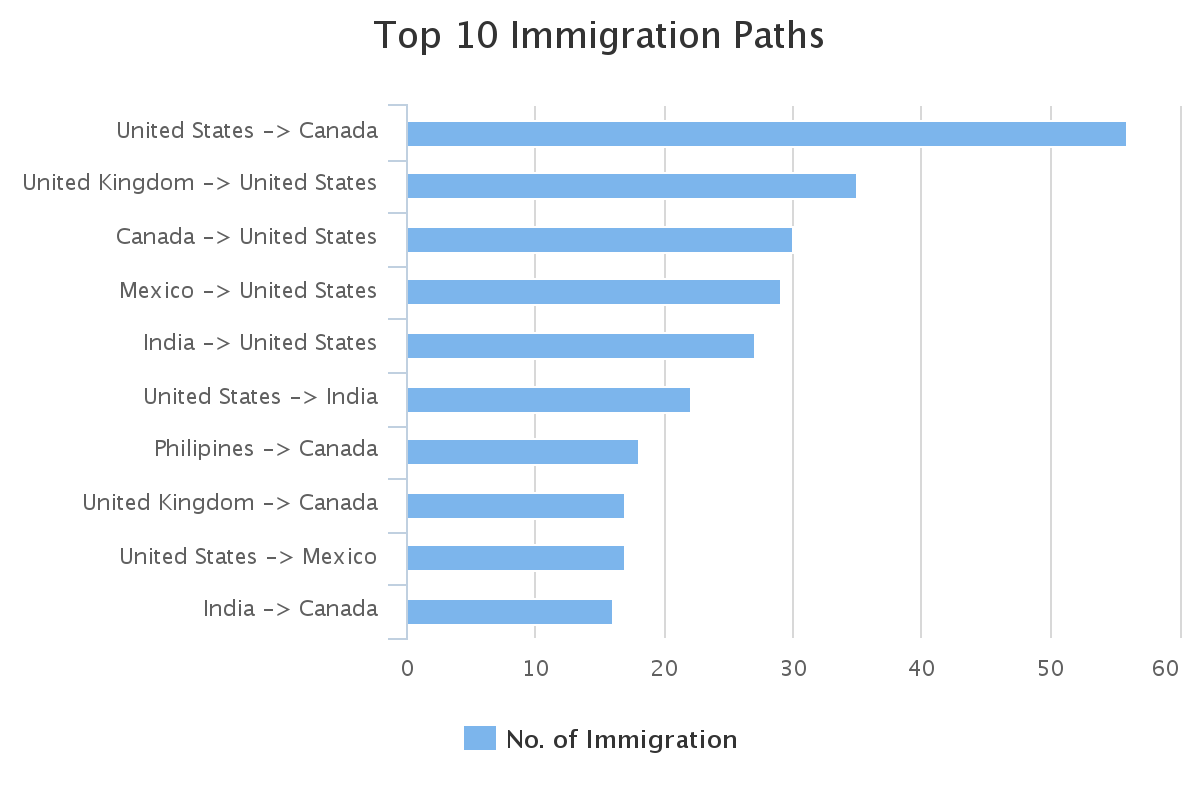
\includegraphics[width=\columnwidth]{Figures/top10routes.png}}
\caption{Top 10 paths of immigrations in identified immigrants}
\label{imm_path}
\end{center}
\vskip -0.2in
\end{figure} 


Our data collection brings us to two crucial questions; 

\begin{enumerate}
    \item How accurate is our results? Have the identified immigrants actually made an immigration?
    \item How does our set of identified immigrants represent the actual demography of the immigrants? Have we made a good sample for our data analysis?
\end{enumerate}

To address the first question we manually analyzed the profiles of a random selection of ten users of the identified immigrants. We could confirm the immigration for seven of them as it clearly showed signs of immigration in their profiles and the texts of their tweets. The other 3 did not show immigration sings nor was it clear that they actually have not made an immigration. 

Regarding the second question, we compared the demography of the identified immigrants in term of gender and source country with the demography of actual immigrants in the world. In order to do so we only focused on US immigrants and extracted those identified Twitter immigrant accounts whose destination country was United States. We also used data collected by \cite{ref22} and \cite{ref23} of demography of immigrants in the United States. Figure \ref{demography} shows the comparison between distribution of our identified immigrants with actual immigrants in the US in term of gender, and Table \ref{srcctr} illustrates the same comparison in term of the rank of the source country. Although this comparison only focused on the immigrants to the United States, the results give a rough estimate on how the distribution of identified set of immigrants is compared to the actual demography of the actual immigrants. The comparison could become more accurate if we could get more data from Twitter such as age, education, income, job, etc., however it is not possible. 

\begin{figure}[ht]
\vskip 0.2in
\begin{center}
\centerline{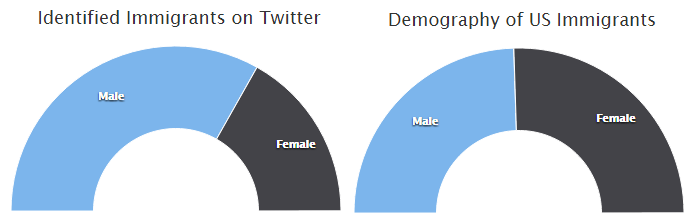
\includegraphics[width=\columnwidth]{Figures/Gender.png}}
\caption{Comparing the diversity of the gender between US actual immigrants and US identified immigrants on Twitter}
\label{demography}
\end{center}
\vskip -0.2in
\end{figure}


\begin{table}[ht]
\centering
\caption{Rank of the source countries of the immigrants to the United States. Comparing the actual demography of the US immigrants with the US immigrants identified on Twitter}
\label{srcctr}
\begin{tabular}{l|c|c}
\multicolumn{1}{c|}{Country} & \begin{tabular}[c]{@{}c@{}}Rank in \\ Identified \\ Immigrants\end{tabular} & \begin{tabular}[c]{@{}c@{}}Rank in \\ Actual \\ Demography\end{tabular} \\ \hline
United Kingdom               & 1                                                                           & 13                                                                      \\
Canada                       & 2                                                                           & 11                                                                      \\
Mexico                       & 3                                                                           & 1                                                                       \\
India                        & 4                                                                           & 3                                                                      
\end{tabular}
\end{table}

\section{Tweets Sentiment Analysis}

In order to investigate the mood expressed on the tweets we built a classifier trained by Logistic Regression to analyze the sentiment of the tweets in terms of three class labels; dejection, anxiety, and hostility. 

\subsection{Training the Classifier}

The training data that we used to train the classifier is a set of 2367 manually labeled tweets for the three desired class labels. 31.4\% of the tweets in our training data have a positive label for at least one of the class labels i.e. dejection, anxiety, and hostility. Figure \ref{training} illustrates how our training data is distributed between the classes. 

\begin{figure}[ht]
\vskip 0.2in
\begin{center}
\centerline{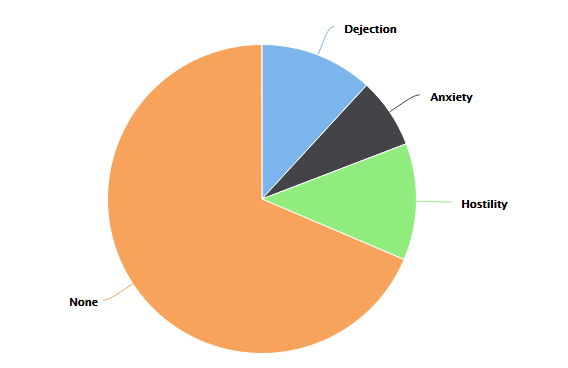
\includegraphics[width=\columnwidth]{Figures/training.PNG}}
\caption{Distribution of the class labels in the training data}
\label{training}
\end{center}
\vskip -0.2in
\end{figure}

In order to evaluate the performance of our classifier we used a 10-fold cross validation and Table \ref{accuracies} shows values in regards to the accuracy of the classifier. 

\begin{table}[]
\centering
\caption{Accuracies for the classifier trained by each class label}
\label{accuracies}
\begin{tabular}{clll}
\hline
\multicolumn{1}{l}{} &  & \begin{tabular}[c]{@{}l@{}}Positive\\ Class\end{tabular} & \begin{tabular}[c]{@{}l@{}}Negative\\ Class\end{tabular} \\ \hline
\multicolumn{1}{c|}{\multirow{4}{*}{Dejection}} & Precision & 0.9843 & 0.9445 \\
\multicolumn{1}{c|}{} & Recall & 0.6829 & 0.9979 \\
\multicolumn{1}{c|}{} & F-measure & 0.3778 & 0.9226 \\ \cline{2-4} 
\multicolumn{1}{c|}{} & Accuracy & \multicolumn{2}{c}{86.27\%} \\ \hline
\multicolumn{1}{c|}{\multirow{4}{*}{Anxiety}} & Precision & 0.9848 & 0.9424 \\
\multicolumn{1}{c|}{} & Recall & 0.6824 & 0.9979 \\
\multicolumn{1}{c|}{} & F-measure & 0.3141 & 0.9729 \\ \cline{2-4} 
\multicolumn{1}{c|}{} & Accuracy & \multicolumn{2}{c}{84.62\%} \\ \hline
\multicolumn{1}{l|}{\multirow{4}{*}{Hostility}} & Precision & 0.9867 & 0.9811 \\
\multicolumn{1}{l|}{} & Recall & 0.6506 & 0.9990 \\
\multicolumn{1}{l|}{} & F-measure & 0.2809 & 0.9521 \\ \cline{2-4} 
\multicolumn{1}{l|}{} & Accuracy & \multicolumn{2}{c}{91.04\%} \\ \hline
\end{tabular}
\end{table}

\subsection{Results}

Using the Logistic Regression classifier we got the probability of each class label for every tweet of each identified immigrant. Then we focused on the dejection class and calculated the average probability of all the tweets for each immigrant once for the tweets made before his or her immigration and once for the tweets made after the immigration. Figure \ref{dejdiff} illustrates the difference between the average probability of dejection after the immigration and before the immigration for those immigrants in which this difference is more than 1\%. The result indicates that the dejection expressed in tweets has generally increased in average after the immigration for most number of identified immigrants. 

\begin{figure}[ht]
\vskip 0.1in
\begin{center}
\centerline{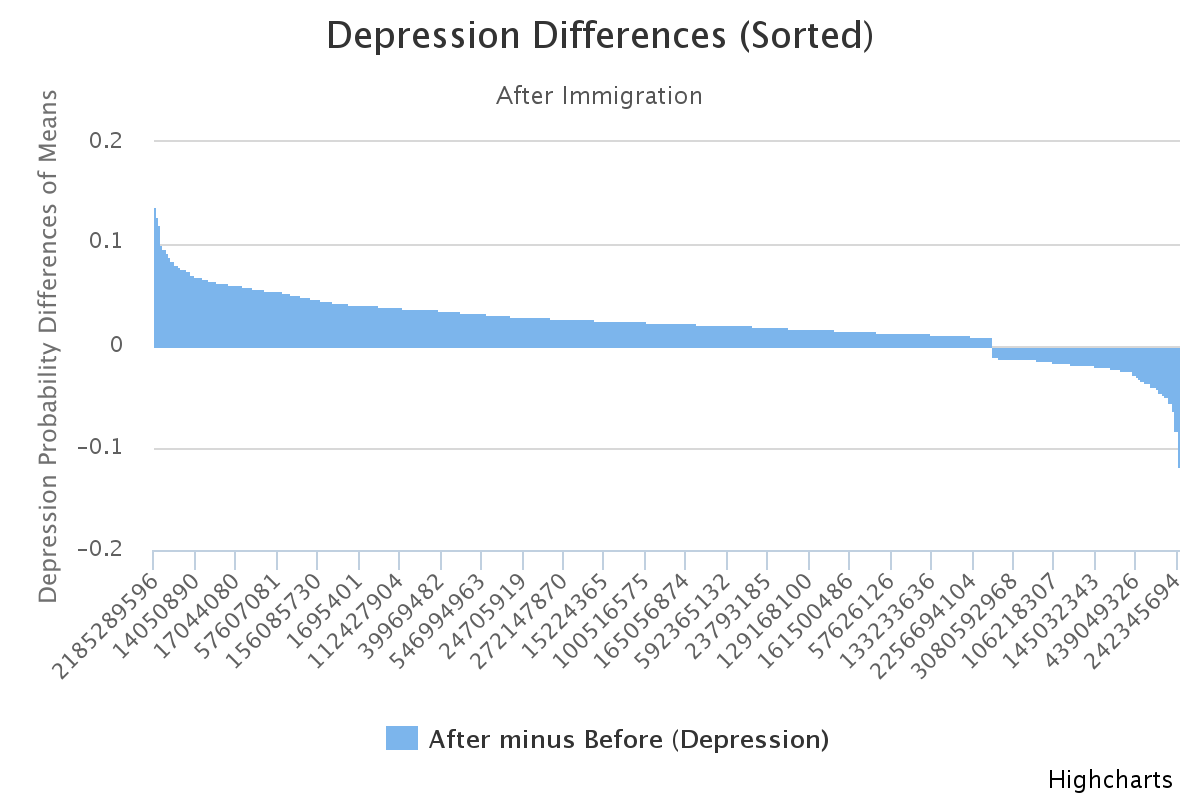
\includegraphics[width=\columnwidth]{Figures/DejectionDiff.png}}
\caption{Distribution of the class labels in the training data}
\label{dejdiff}
\end{center}
\vskip -0.2in
\end{figure}

\section{Difference-in-Differences Analysis}

Difference-in-differences (DD) analysis is a popular method in economics, statistics, and quantitative research to estimate causal relationships. This section describes how we utilized this technique to verify our findings. We identified one similar user account who has not made any immigration for each identified immigrant that has the same gender and is from exactly the same country and has a similar features set that contains rate of tweets 200 days before the immigration, rate of replies (user mentions) 200 days before the immigration, and date of account creation. In order to evaluate the similarity we used co-sine similarity. As a result we have a set of similar non-immigrant twitter accounts as many as the identified immigrants. The next step is to use our classifier to measure the probability of every tweet from 200 days before the immigration to 200 days after the immigration for each user and calculate the average trend for all the users once for immigrants and once for similar non-immigrants. Figure \ref{diffindiff} illustrates the comparison of the trends for each class label between the immigrants and their corresponding similar non-immigrants. The result shows a slight increase in hostility, dejection, and anxiety in immigrants while the similar users experienced a flat trend. 

\begin{figure}[ht]
\vskip 0.1in
\begin{center}
\centerline{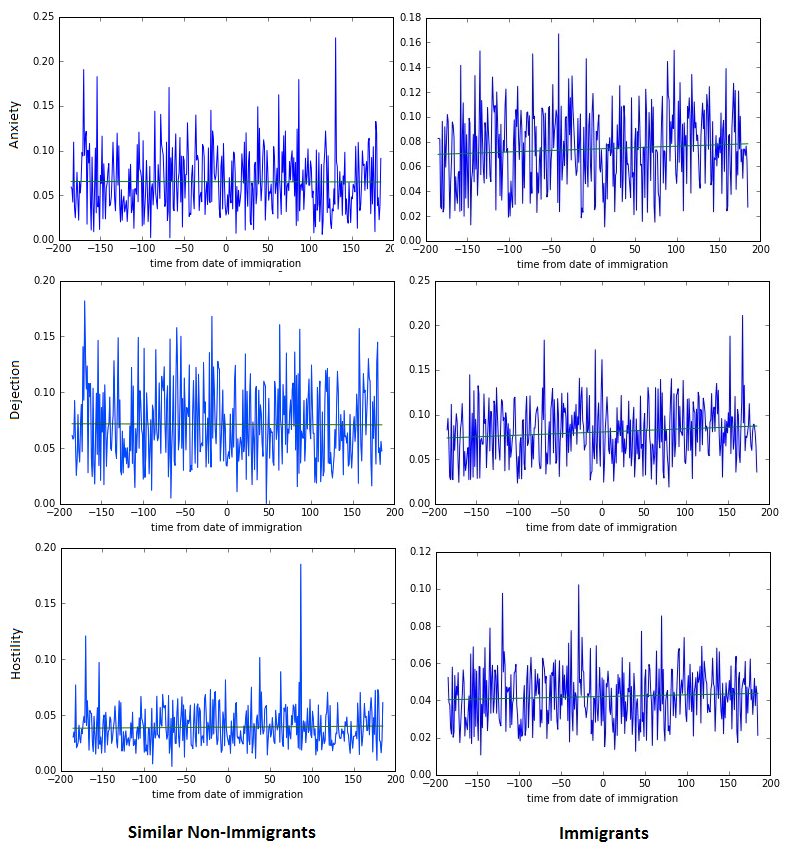
\includegraphics[width=\columnwidth]{Figures/diffindiff.png}}
\caption{Difference in Differences analysis: The trend for each class label before and after the immigration in both immigrants and their similar accounts. }
\label{diffindiff}
\end{center}
\vskip -0.2in
\end{figure}

Finally, we get the mean value for all the probabilities of all the tweets made before and after immigration by all users (once for immigrants and once for similar non-immigrants). Figure \ref{totalmean} shows that the difference between the values achieved for the immigrants is not significant with the values achieved for their similar non-immigrants. The difference value is 0.000793393 and does not seem to be significantly different from zero (given the size of the variance).


\begin{figure}[ht]
\vskip 0.1in
\begin{center}
\centerline{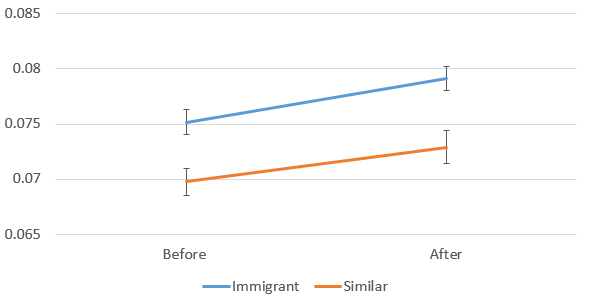
\includegraphics[width=\columnwidth]{Figures/totalmean.PNG}}
\caption{Total Mean of dejection probablity for All before and after immigration}
\label{diffindiff}
\end{center}
\vskip -0.2in
\end{figure}



\section{Conclusion and Future Work}

In this project we successfully identified a set of Twitter accounts who have made an immigration from one country to another. Using sentiment analysis with a Logistic Regression model we classified their tweets based on three class labels; dejection, anxiety, and hostility. Our results indicated an slight increase in all class labels after the immigration. 

Potential future work for this project includes but are not limited to: 

\begin{enumerate}
    \item Focus on individual countries and investigate how immigrants to that particular country has changed their mood expressed on their tweets. 
    \item Include more meta-data of the tweets such as number of retweets and URL share. This could potentially indicate sense of sociability on Twitter by users. We can then study the how more or less socialized the person became after the immigration. 
    \item Repeat the process on data collected in other social network such as Facebook.
\end{enumerate}


\section{Acknowledgement}

I would like to express my sincere thanks of gratitude to Dr. Aron Culotta who gave me this wonderful opportunity to work on this exciting project. I am very thankful to Dr. Culotta for his invaluable feedback, comments, and insights that led to many improvements in the finished product. 

I was also fortunate enough to get detailed feedback from Dr. Shlomo Argamon who kindly spent his precious time on reviewing my project. I sincerley thank Dr. Argamon for helping me on this project. 

Additionally, I would like to thank Virgile Landeiro who generously shared his manually labeled training data with me and helped me throughout the project. 

\bibliography{example_paper}
\bibliographystyle{icml2015}

\end{document} 


